\newpage
\section{Chancen und Risiken}

\begin{figure}[H]
\caption{Unterschied der Platformen}
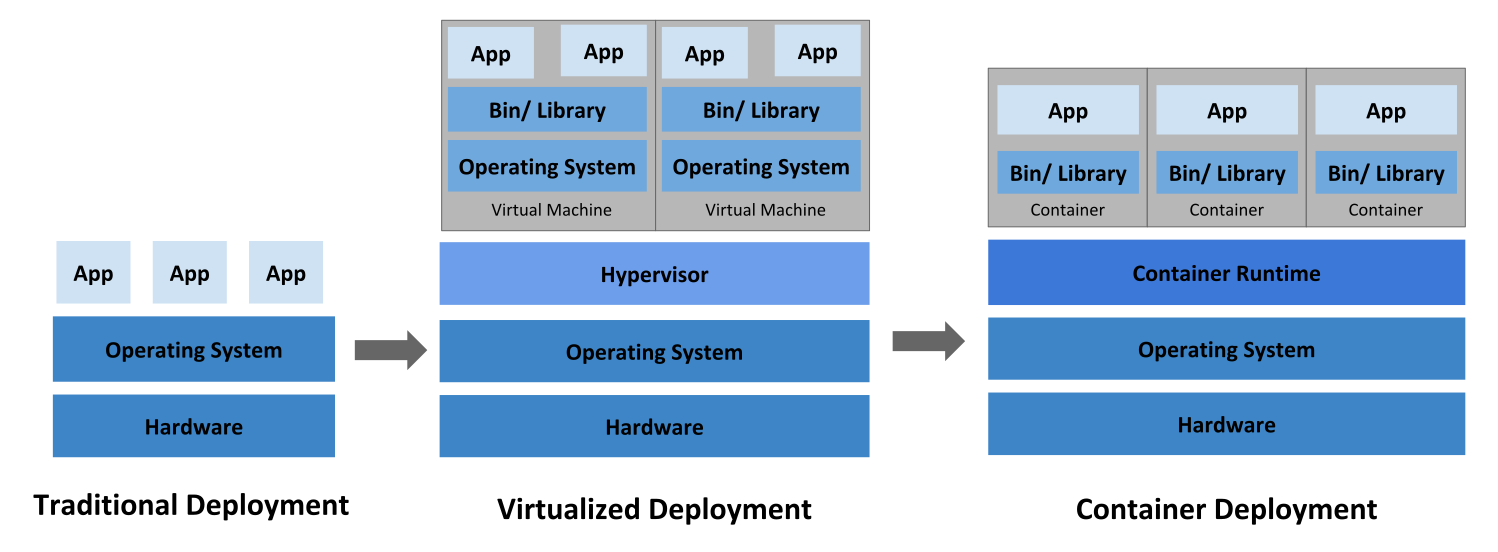
\includegraphics[width=0.9\textwidth]{container_evolution}
\\
\cite[][27.03.2020]{Quelle: https://bit.ly/32EnzVe}
\end{figure}

Mit jedem der genannten Konzepte wird das Ziel verfolgt eine App zu starten sowie diese dann erreichbar zu machen, der Öffentlichkeit oder ausgewählten Personen.
Schon genannte Aspekte die zu beachten sind währen die Ausfallsicherheit sowie Einfachheit des Arbeitens.

Die erklärten Möglichkeiten der Skalierung währen mit allen Konzepten anwendbar, jedoch wird klar das mittels der Kontainerisierung dies am schnellsten machbar währe.
Während bei Bare-metal oder Virtualisierung ein weiterer Server/VM erstellt und eingerichtet werden muss, muss bei Docker nur ein Befehl ausgeführt werden um innerhalb Sekunden eine zweite 
Instanz der App hochzufahren.
Darüber hinaus ist ein wichtiger Faktor das bei den Wegen ohne Docker Fehler passieren können. Fehler, die auch vielleicht erst irgendwann während der Benutzung auffallen.
Zum Beispiel wenn die falsche Version einer Abhängigkeit installiert wird, oder Dateien an die falsche Stelle kopiert werden.

Diesen Faktor der Fehleranfälligkeit ist bei der Containerisierung komplett irrelevant, denn ein Docker Image ist unveränderbar, und wenn es gestartet wird 
entstehen immer exakte Kopien.

Zeit ist in jedem Unternehmen eine kostbare Währung. Wie bereits erwähnt zieht man mittles Kontainerisierung in Sekunden eine neue Instanz jedlicher Server hoch.
Dies ist mittlerweile ähnlich bei Virtualisierung auch möglich, dort wird mit Kopien von VM's gearbeitet. Bedeutet, das eine VM mit Betriebssystem präperiert wird, und
sobald dann eine weitere Instanz mit dem OS benötigt wird dupliziert man die vorgefertigte Maschine. Dadurch spart man den Schritt der Neuerstellung und Einrichtung, jedoch
ist dies in keinster im Sekundenrahmen, und in den meisten Fällen muss die VM die kopiert werden soll ausgeschaltet sein damit sie kopiert werden kann. 
Dies würde bei einer Website bedeuten das man sie offline nehmen muss, um die Kopierfähigkeit auszunutzen.
Bare-Metal hat kaum Möglichkeiten gut ein System zu duplizieren der nicht mit viel händischer Arbeit verbunden wäre.

Soviel dazu, nur muss ja wie schon bereits erwähnt muss um Skalieren zu können ein Proxy vor allen verfügbaren Instanzen stehen, damit eine Adresse auf alle zeigen kann.
Dieses Prinzip trifft auf alle Bereitstellungskonzepte gleich zu, jedoch wurde mittels der Software Kubernetes diese Arbeit erheblich erleichtert. Auch die Skalierung
wird auf eine neue Ebene gehoben.

Nun sind die hauptsächlichen Chancen und Risiken der verschiedenen Platformen bekannt, jedoch hat die Containerisierung aufgrund ihrer 
unveränderlichen Images sowie Geschwindigkeit noch weitere Möglichkeiten die die anderen Platformen nicht so leicht bieten können.

\subsection{Kubernetes}

\begin{figure}[H]
\caption{Kubernetes Logo}
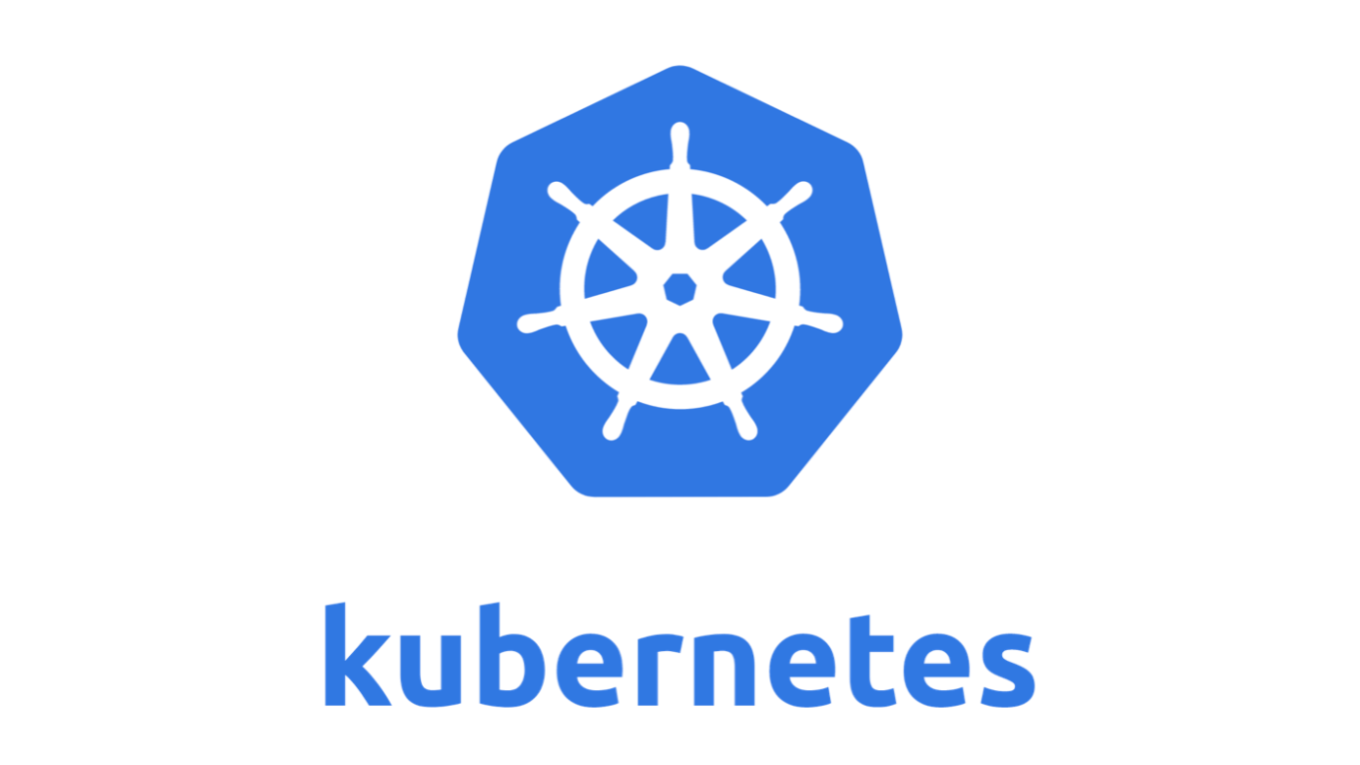
\includegraphics[width=0.7\textwidth]{kube}
\\
\cite[][27.03.2020]{Quelle: https://bit.ly/3afiIMv}
\end{figure}

Kubernetes, oder kurz K8s, ist ein von Google gestartetes Open Source Projekt unter der Apache-2.0 Lizens. Dies bedeutet, das die Software von jedem verwendet sowie angepasst werden, 
jedoch nicht unter einer anderen Lizens weitervertrieben werden darf. Mittlerweile hat der Quellcode, welcher auf der Codeversionierungsplatform Github veröffentlicht ist, über 2400 Mitentwickler.
Jeder kann nämlich Anpassungen vornehmen und diese in das Repository, der Speicherort auf Github, einfliesen lassen. Dies geschiet jedoch nur, wenn die Anpassung
vorher durch verschiedene Tests sowie Abnahmen von anderen Mitarbeitern bestätigt wurde.

K8s baut wie erwähnt auf der Kontainerisierung auf. Im Grunde kümmert es sich um das Verwalten von Containern und übernimmt für uns das Starten und Stoppen.
Erstmal ist K8s aber eine Software die für das Clustering gebaut ist, bedeutet den Verbund von mehreren verschiedenen Servern zu einem. Durch einen solchen Verbund sind nicht nur mehr Ressourcen verfügbar,
sondern auch eine gewisse Ausfallsicherheit gegeben. Sollten die einzelnen Knoten, eigene Maschinen im Verbund, jedoch virtualisiert auf einer physikalischen Maschine laufen, kann ein Hardwaredefekt natürlich immernoch
alles zum erliegen bringen.
Das Clustering sieht so aus, das es in einem Verbund eine gewisse Anzahl sogenannter Master-Knoten und eine Anzahl Worker-Knoten gibt. Der Unterschied ist der, das nur auf den Worker-Knoten
die Container die ausgeführt werden sollen gestartet werden, während sich die Master Knoten nur um das Controlling kümmern.

Was hinter diesem Controlling steckt ist der Kernpunkt von K8s. Ein K8s Cluster kann nämlich erstmal unendlich viele Worker-Knoten, in Zukunft nur noch Nodes genannt, haben. Um diese zu steuern braucht es mindestens
einen Master-Knoten, in Zukunft nur noch Master. Der Master weiß über alle ihm zur Verfügung stehenden Nodes bescheid, und kann Metriken wie Ressourcenverbrauch abfragen. Die Nodes warten nur auf Befehle vom Master.
Für einen hochverfügbaren K8s Cluster benötigt man mehr als einen Master, sowie mindestens zwei Nodes. Nodes nehmen Befehle von allen Mastern entgegen, genauso wie alle Master auch im Austausch über ihre Befehle stehen.

Wenn nun eine App die durch beispielsweise Docker schon Containerisiert wurd gestartet werden soll, gibt man diese Anweisung an einen der Master. Der Master kümmert sich dann darum das diese App gestartet wird.
Dazu schaut der Master auf welcher seiner Nodes noch genug freie Ressourcen zur Verfügung stehen, und gibt dann den Befehl an die Node weiter das das Docker Image zu starten. Dazu muss das Image
auf einen externen Server hochgeladen sein, den jeder der Nodes muss über das Internet das Image runterladen können. Dazu gibt es sogenannte Docker Registries, in denen man mittels dem Docker Client
sehr leicht Images hochladen kann.
Damit der Master weiß wieviele Ressourcen auf der Node frei sein müssen damit die App überhaupt starten kann, werden Angaben zu Mindestanforderungen sowie auch Höchstanforderungen mitgegeben. Wenn diese 
nicht mitgegeben werden, startet der Master den Container einfach auf einem zufälligen Node der noch ein bisschen Platz hat.

Der Vorteil von dieser Weise ist der, das die Nodes die dem Cluster angehören zum einen flexibel hoch- und runterskaliert werden können. Man kann also mit der Anzahl der Apps mitwachsen, und muss nicht von vornherein die ganze Hardware
für den K8s Cluster aufwarten. Zweitens können Nodes aber auch an verschiedenen Standorten laufen. Solange die Master mit ihnen über das Internet sprechen können ist der Standort egal.
Heutzutage kann schnell über einen der Cloud-Dienste wie Amazon Web Services oder Google Cloud Platform weitere Hardware auf Minutenbasis gebucht werden. Wenn zum Beispiel ein Onlineshop sich auf einen
Ansturm durch eine Verkaufsaktion vorbereiten will, kann er einfach weitere Hardware buchen und seinen K8s Cluster hochskalieren, und nach dem Ansturm wieder herunterfahren.

Die Master übernehmen nicht nur die Verteilung der Docker Container, sie überwachen und messen durchgehend alle möglichen Daten, wodurch weitere Funktionalitäten möglich geworden sind.
Beispielsweise das automatische horizontale Skalieren von Docker Containern. Sollte der Master merken das die Last oder der Traffik auf einen Container zu hoch ist, startet K8s für uns einen weiteren Container der gleichen Sorte. 
Dieser kann wieder auf jeder Node gestartet werden, also auch auf der gleichen wie der erste Container, muss es aber nicht.
Wie schon beschrieben sollte nachher aber nur eine Adresse angesprochen werden, um auf einen der Replikate des Docker Containers zu kommen. Dazu hat K8s das eingebaute Feature Services. Ein K8s Service ist ein Verbindungsglied
von allen Containern einer Sorte zu einer Adresse. Man kann von einem Loadbalancer sprechen. Dieser Service kann von dem öffentlichen Netz angesprochen werden. Ein Service ist über alle Nodes gespannt, sodass die 
Replikate des Containers auf jeder Node laufen können, und der Service dennoch alle von ihnen erreicht.

Zusammengefasst kann durch einen K8s Cluster zum einen die wirkliche Hardware flexibel hoch und runter skaliert werden, und das auch regionenübergreifend, und zum anderen können und die K8s Automatismen die Skalierungsarbeit unserer App abnehmen.
Wenn man das DevOps Prinzip hier anbringt, dann ist der wirkliche K8s Cluster, also das Aufsetzen und Warten dieses, der Aufgabenbereich der Ops, und das Benutzen dessen die Aufgabe der Devs.
Ein Ops hat somit nicht mehr eine wachsende Anzahl einzelner Server die einzeln gepflegt werden müssen, sondern nur noch eine einzige Platform für alle auszuführenden Apps.

Kubernetes bietet also erhebliche Vorteile gegenüber anderen Platformen, jedoch ist es auch eine neue Stufe der Komplexität.
Ein Ops muss sich in die neue Technologie erst einarbeiten. Dazu zählt erst einmal die Container Engine, zu meist Docker, zu verstehen.
Jedoch ist dies auch die kleinste Hürde, den auch wenn das Prinzip von K8s zwar leicht verständlich ist, sieht die Umsetzung etwas komplizierter aus.
Dazu kommt auch, das sich die Software ständig weiterentwickelt, und man immer dazulernen muss. Im Jahr kommen mehrere neue Releases raus, wodurch 
auch der Updateaufwand des Clusters nicht unerheblich ist. Generell kommt zum Überwachen und Warten noch einiges an Software hinzu die ein Ops beherschen muss um 
den Cluster ordentlich zu Überwachen.
Dies ist jedoch wichtig, denn wenn die Master beispielsweise ausfallen, sind die meisten Dienste die im Cluster laufen nciht mehr erreichbar, was einem Hardwaredefekt bei einer einzelnen Maschine gleichkommt.
Jedoch sei auch gesagt, das das Clustering einen gewaltigen Vorteil bringt. Sollte eine Node ausfallen, fallen auch alle darauf laufenden Container aus. Jedoch werden die Master dies bemerken, 
und versuchen auf den anderen verfügbaren Nodes alle Container wieder neu zu starten. Dadurch kommt es maximal zu einem kurzen Ausfall eines Dienstes, und sollte dieser mehrere Replikate auf verschiedenen Nodes haben kommt es sogar zu gar keinem Ausfall.
Ein Ops würde in so einem Fall die kaputte Node endweder reparieren und wieder in den Cluster eingliedern, oder einfach ausschalten und eine komplett neue Node erstellen und dem Cluster anhängen.